%
% 修士学位請求論文(副・正)テンプレート
% MasterThesisSample.tex
% By KASHINA, Yuki (EM-14003)
%
\documentclass{MasterThesis}
%\documentclass[fleqn]{MasterThesis} %数式を左寄せ


%%%%%%%%%%%%%%%%%%%%%%%%%%%%%%%%%%%%%%%%%%
% ユーザ任意のパッケージ
%%%%%%%%%%%%%%%%%%%%%%%%%%%%%%%%%%%%%%%%%%
%\usepackage{booktabs}
%\usepackage{multirow}
\usepackage[dvipdfmx]{xcolor}
\usepackage{otf}


%%%%%%%%%%%%%%%%%%%%%%%%%%%%%%%%%%%%%%%%%%
% マクロ
%%%%%%%%%%%%%%%%%%%%%%%%%%%%%%%%%%%%%%%%%%
%<local definition>
\newcommand{\texcmd}[1]{\texttt{\textbackslash{}#1}}

\usepackage{setspace}
\def\commentary#1{\raisebox{\baselineskip}{\parbox{0.8\textwidth}{\begin{spacing}{0.8}#1\end{spacing}}}\vspace{.42\baselineskip}\endgraf}
%</local definition>


%%%%%%%%%%%%%%%%%%%%%%%%%%%%%%%%%%%%%%%%%%
% ルートパス
%%%%%%%%%%%%%%%%%%%%%%%%%%%%%%%%%%%%%%%%%%
\graphicspath{{figure/}}
\tablepath{{table/}}


%%%%%%%%%%%%%%%%%%%%%%%%%%%%%%%%%%%%%%%%%%
% 行間調整
%%%%%%%%%%%%%%%%%%%%%%%%%%%%%%%%%%%%%%%%%%
\renewcommand{\baselinestretch}{1.0}


%%%%%%%%%%%%%%%%%%%%%%%%%%%%%%%%%%%%%%%%%%
% 図表キャプションの接頭辞
%%%%%%%%%%%%%%%%%%%%%%%%%%%%%%%%%%%%%%%%%%
%\renewcommand{\jfigurename}{図}
%\renewcommand{\jtablename}{表}
%\renewcommand{\efigurename}{Fig.~}
%\renewcommand{\etablename}{Table~}


%%%%%%%%%%%%%%%%%%%%%%%%%%%%%%%%%%%%%%%%%%
% フォントサイズ
%%%%%%%%%%%%%%%%%%%%%%%%%%%%%%%%%%%%%%%%%%
%%% 英文タイトル
%\renewcommand{\etitlefontsize}{\fontsize{21pt}{21pt}}
\renewcommand{\etitlefontsize}{\fontsize{14pt}{14pt}}

%%% 本文
%\renewcommand{\mainfontsize}{\fontsize{14pt}{25pt}}
\renewcommand{\mainfontsize}{\fontsize{12pt}{21pt}}

%%% キャプション
%\renewcommand{\captionfontsize}{\fontsize{14pt}{17pt}}
\renewcommand{\captionfontsize}{\fontsize{11pt}{14pt}}


%%%%%%%%%%%%%%%%%%%%%%%%%%%%%%%%%%%%%%%%%%
% 書誌情報
%%%%%%%%%%%%%%%%%%%%%%%%%%%%%%%%%%%%%%%%%%
%%% 和文タイトル
% \newlineで改行,数式やコマンド,クォートは{}でグルーピング
% \jtitle{体験情報に基づくLies-Bias型観光支援システム}{}
\jtitle{ユーザの体験情報を用いた観光支援システム}{}

%%% 英語タイトル・サブタイトル
% \etitle{ユーザの訪問情報を用いた観光支援システム}{}

%%% 所属専攻 //工学研究科は不要
\affiliate{情報学専攻}

%%% 氏名・学籍番号 //\ruby{漢字}{かん|じ}, 性名間に半角空白を挿入
\author{\ruby{潘}{はん}~\ruby{健太}{けん|た}}

%%% 指導教官名・指導教官役職 //姓名間に半角空白を挿入
\supervisor{北山~大輔}{准教授}

%%% 修了年月(西暦) //全角を推奨
\ptdate{2020}{3}

%%% 前文のタイトル
\abstractname{要旨}{Abstract}

%%% 目次の有効化
\toctrue

%%% 図目次の有効化
\loftrue

%%% 表目次の有効化
\lottrue

%%% 索引の有効化
%\makeindex

%%% 研究室内部資料セクション(付録)の有効化
%\domestictrue



%%%%%%%%%%%%%%%%%%%%%%%%%%%%%%%%%%%%%%%%%%
% 書誌情報の設定終了
%%%%%%%%%%%%%%%%%%%%%%%%%%%%%%%%%%%%%%%%%%
\eom



%%%%%%%%%%%%%%%%%%%%%%%%%%%%%%%%%%%%%%%%%%
% 前文(和文)
\jabstract
%%%%%%%%%%%%%%%%%%%%%%%%%%%%%%%%%%%%%%%%%%


%%%%%%%%%%%%%%%%%%%%%%%%%%%%%%%%%%%%%%%%%%
% 本文の開始
%%%%%%%%%%%%%%%%%%%%%%%%%%%%%%%%%%%%%%%%%%
\main



%%%%%%%%%%%%%%%%%%%%%%%%%%%%%%%%%%%%%%%%%%
\chapter{序論}
%%%%%%%%%%%%%%%%%%%%%%%%%%%%%%%%%%%%%%%%%%
一般に,ユーザは観光旅行する前にWeb上の情報やガイドブックを活用して計画を立てることが多くなっている.
その際,目的とする観光スポットに関する概要やアクセスするための方法などの情報を集める.
ガイドブックは,有名な観光スポットや流行りのものに焦点を当て,そのスポットの料金や見どころ,そして食べ物などが掲載されており,その土地に初めて観光で訪れるユーザや,普段から頻繁に観光旅行をしないユーザにとって満足を得られるような内容が書かれている.そのため,ガイドブックは普段から頻繁に観光旅行をするようなユーザや,その観光スポットに対してこだわりの観点を持つユーザの個別の嗜好までは考慮できない.

Web上の情報に関して,観光スポットに関する総合的な情報が掲載された公式サイト,過去にそこを訪れた観光者による旅行記ブログサイト,そして,評価が記載されたレビューサイトなどの様々なサイトがある.
しかしながら,種々のサイトが混在しており,膨大な情報から自分の嗜好に合う観光スポットの情報を得ることは簡単ではない.
目的の情報を収集するためには手動で閲覧し取捨選択しなければならない.
旅行計画を立つために,まず訪問したいエリアを決定する必要がある.
その後,観光スポット検索サイトやガイドブックの観光スポット情報を調べて観光スポットを決定する.
ユーザの意識決定の材料の1つとして,るるぶトラベル\footnote{https://www.rurubu.travel/},Tripadvisor\footnote{https://www.tripadvisor.com/}やじゃらん\footnote{https://www.jalan.net/kankou/}などの観光スポット検索サイトがある.これらのサイトには特定の観光スポットを訪問したことのあるユーザがレビューを投稿し,観光スポットに関する豊富な情報が存在している.
観光スポット検索サイト上で観光スポットに付与される情報の例\footnote{https://www.jalan.net/kankou/130000/?screenId=OUW2201}を図\ref{fig:観光スポット検索サイト上で観光スポットに付与される情報例}に示す.
なお,これらの情報のうちユーザレビュー以外の情報(概要文・タグ・評価点など)はメタデータと呼ばれる.
\begin{figure}[t]
    \centering
    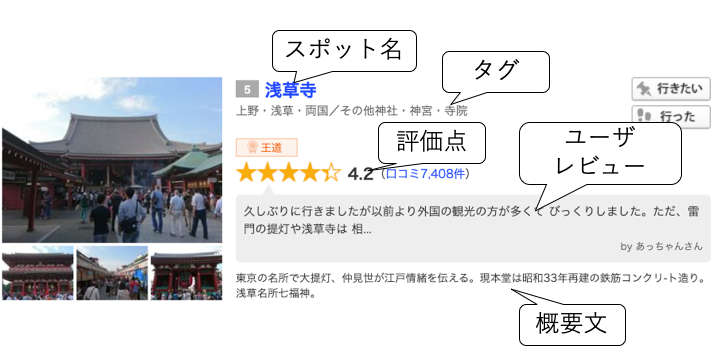
\includegraphics[width=0.9\textwidth]{./figure/spot_info.png}
    \caption{レビューサイト上で観光スポットに付与される情報例}
    \label{fig:レビューサイト上で観光スポットに付与される情報例}
\end{figure}

観光スポット検索サイトに掲載された情報を基に,利用者(ユーザ)は自身の嗜好や目的に合致した特徴を持つ対象観光スポットを検索する.
多くの観光スポット検索サイトでは,対象観光スポットに付与されるメタデータを利用した以下のような検索方法が提供されている.

\begin{itemize}
\item ユーザが指定したタグを持つ対象観光スポット
\item 評価点などの数値メタデータに基づく並び替え
\item 入力単語(クエリ)を概要文中に含むオブジェクトの検索
\end{itemize}

しかし,これらのメタデータを用いた検索方法だけでは検索が困難な場合も存在する.
たとえば,対象観光スポットを実際に利用することでユーザが得られる印象・感情・体験などを表す特徴に基づき対象観光スポットを検索したい場合などが該当する.
また,訪問したいエリア内に数多くの観光スポットが存在している.
ユーザは検索エリアに関する事前知識がないため,検索された多数の観光スポットからどの観光スポットのレビューを読むべきか効率的に判断することは困難で,自身のイメージから外れない観光スポットを見つけることは容易ではない.
そこで,本研究では,さまざまな観光スポットを効果的に理解するためには,ユーザが訪問した体験のある観光スポットとを使って未訪問スポットを検索する手法を提案した.
観光支援システムを構築するにあたり課題となる点は2つ説明する.

\begin{enumerate}
\item 観光スポット間の対応付け

ある観光スポットに対応する観光スポットを判定する手法として,レビューやカテゴリが類似したコンテンツであるという観点で判定する方法が一般的である.
観光スポットで用いられる単語に対する従来の特徴量TFIDFは,観光スポット内での重要な単語を判定する際に用いられる.
しかし,従来手法のTFIDFはユーザの観光スポット選択における意図や他スポットへの関心について考慮されていない.
そのため,ある観光スポットが他の観光スポットと比較するとき,その観光スポットの特徴を表すことができない.
そこで,あるスポットに対し,既に訪問した観光スポットと比較した相対的特徴ベクトルを作成し,相対的特徴ベクトル間の類似度に基づいて既訪問スポットと未訪問スポット間の対応付け手法を提案する.第3章で,より具体的な提案手法について述べる.

\item 観光スポットの対応関係を地図上に可視化

地理的情報の可視化を意味的な関係の可視化に取り込む情報の可視化としては,抽出した情報を地図上にマッピングするのが一般的である.また,意味的な関係性の可視化として,グラフモデル上でオブジェクト間のつながりを関連度で表現することが多い.
観光スポット間の意味的な対応関係を可視化するために,未訪問スポットは地図上で実在する座標に固定され,配置の自由があるのは既訪問スポットのみという制約がある.
そこで,ある未訪問スポットに対して,入力した既訪問スポットがどのような関係にあるのか地図上で,一目で把握できるために,既訪問スポットと未訪問スポットの対応関係を可視化する手法を提案する.第4章で,より具体的な提案手法について述べる.
\end{enumerate}

以下に本論文の構成を示す.
ます,2章で本研究のアプローチについて述べる.
ここでは観光支援システムのアルゴリズムと関連研究について述べる.
この観光支援システムのための2つの観点に基づく各手法は3章と4章で述べる.
3章では,ユーザの既訪問スポットの位置付けに基づく未訪問スポットの説明手法について述べる.
4章では,地図上における未訪問スポットの説明向上のための観光スポットの対応付け可視化手法について述べる.
5章では,各手法に対する評価実験結果を踏まえた提案手法全体に対する考察を行う.
6章では,まとめと今後の課題を述べる.


%%%%%%%%%%%%%%%%%%%%%%%%%%%%%%%%%%%%%%%%%%
\chapter{本研究のアプローチ}
%%%%%%%%%%%%%%%%%%%%%%%%%%%%%%%%%%%%%%%%%%
\section{観光支援システム}
% 観光支援システムの1つに,求める情報の発見までにかかる手間を削減することが考えられる.
観光支援システムの1つに,求める観光スポット情報を発見するために観光スポットの理解をしやすくすることが考えられる.
観光情報収集までの過程を効率化することで,ユーザの観光計画への敷居は下がり,訪れたことない観光スポットの理解の向上も望める.
本節では,ユーザいままで体験したことがありかつ気に入った観光スポットを利用し,訪問したいエリア内の観光スポットに対して関連付けすることで,手軽に観光情報を理解する観光支援システムを提案する.
観光支援システムの具体的な流れを図\ref{fig:観光支援システムの流れ}に沿って説明する.
\begin{figure}[t]
    \centering
    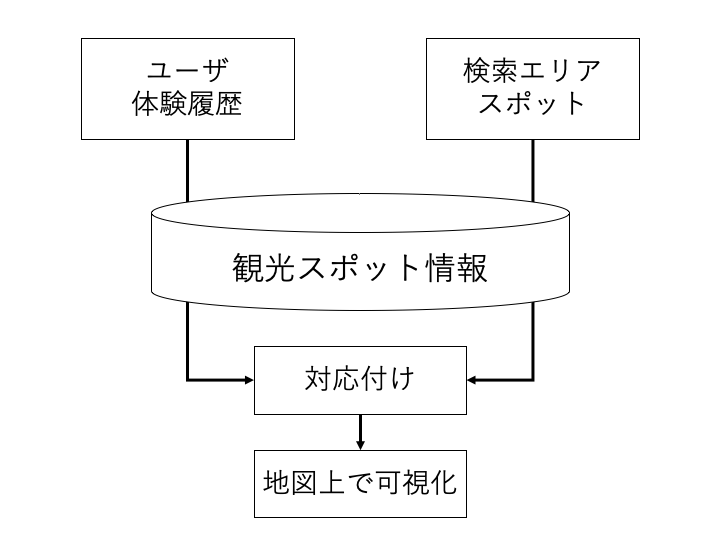
\includegraphics[width=0.9\textwidth]{./figure/system_fig.png}
    \caption{観光支援システムの流れ}
    \label{fig:観光支援システムの流れ}
\end{figure}

まず,ユーザの体験履歴の中ていままで訪れたことがあるかつ気に入った観光スポットを入力する.
次に,これから行ってみたい都道府県やエリアを入力する.
そして,データベースで保存されている2016年10月までのじゃらんの観光スポットレビューデータを使って提案手法に適用することで,ユーザの未知な観光スポットに対する理解を支援するため,既に訪問したことがある観光スポットの特徴を用いて,未訪問エリアの観光スポットを説明するために対応付けを行う.

本研究における観光スポットの対応付けに関して,ユーザによって,その強調するべき特徴が変化する.
たとえば,日本の有名な観光スポットを履歴に持つユーザにとっての「東京都庁舍展望台」と「金閣寺」について考える.
このとき,「金閣寺」の相対的特徴は,お寺,金色,京都などである.
「東京都庁舍展望台」の相対的特徴は,展望,夜景,建物,新宿などが考えられる.

一方,京都の寺院を履歴に持つユーザにとっての「金閣寺」と「清水寺」について考える.
このとき,同じ「金閣寺」でもお寺や京都などは特徴にはならず,「金閣寺」の相対的特徴は,金色,金箔,輝きなどとなる.
「清水寺」の相対的特徴は,舞台や一望などである.

対応付けを行ったなあと,ユーザに未訪問スポットを説明するための観光スポット特徴語を抽出する.
最後に,地図上で既訪問スポットと未訪問スポットの対応関係と特徴語を可視化することで,ユーザが未訪問スポットに対する理解を容易化することを目指さす.

%%%%%%%%%%%%%%%%%%%
\section{関連研究
}
%%%%%%%%%%%
\subsection{体験履歴による検索や推薦システムに関する研究}
倉島ら\cite{Kurashima}は,Flickrに投稿された写真のジオタグ情報を人々の旅行履歴として利用した旅行ルート推薦手法を提案した.この手法では,ユーザの現在地から行きやすい場所とユーザの興味に合致した場所に移動しやすいと仮定し,行動モデルを生成している.
ユーザのジオタグ付き写真集合は,時間情報でソートすると個人の旅行履歴とみなすことができると考え,ジオタグ情報を利用してユーザの行動モデルを生成している.

Chengら\cite{Cheng}は,自由に利用できるコミュニティ投稿の写真を活用して,パーソナライズされた旅行のおすすめに焦点を当て,特定のユーザプロファイルまたは属性を考慮し,パーソナライズされた旅行の推奨を行うことを提案した.

観光地検索するとき,松本ら\cite{松本}はクチコミから特徴 語を抽出して利用する研究を行った.
抽出対象を任意の名詞として,4種類の手法,TFIDF,ATF(Average Term Frequency),ポアソン確率,エントロピーのうちどの手法が特徴語抽出に適しているのか検討を行った.
また,抽出した特徴語を利用した検索支援システムを試作し,実験を通して特徴語提示の効果を検証した.

嶋田ら\cite{嶋田}はWebから観光情報を抽出し,複数の特徴べクトルから観光地間の類似性を評価することで,観光地を推薦するシステムを提案した.
観光地の特徴べクトルは,知恵袋・ブログ上での共起キーワードと時系列分布,知恵袋上でのカテゴリ構造,観光地周辺施設,地図画像から生成した.
これらの特徴べクトルから観光地間の類似度の測定を行い,類似度の高い観光地を推薦した.

廣嶋ら\cite{廣嶋}は地理情報検索の際のクエリ入力支援として,提示する特徴語の抽出手法について研究を行った.
この手法では,各ブログ記事から特徴語候補の抽出および地点の特定を行った.
具体的には,特徴語の候補をWikipediaの見出し語に限定し,ポアソン確率を用いて特徴語抽出を行った.
また,地点の特定のための地名表現の抽出および緯度経度への変換の方法としては平野ら\cite{平野}の手法を用いた.

野守ら\cite{野守}は日本全国の観光地のクチコミデータを用いて,観光客が話題にする観光テーマを確率的に抽出し,そのテーマを軸として各観光地の特徴を定量的に評価した.
また,クチコミのテキストデータにテキストマイニングを実行して表現を抽出し,観光地ごとにその表現の出現頻度を集計したクロス集計表にPLSAを実行することで,観光客のクチコミだけに基づいた観光テーマの抽出と観光地の特徴分析を行なった.

このように多くの研究はユーザに合致する観光スポットの抽出や,一般的な特徴の抽出に焦点をあてているが,本研究では,ユーザの選択性を高めるために,個人化した特徴を抽出する点では異なる.

% 佐藤\cite{佐藤}はコスメアイテムに対してのクチコミからアイテムの特徴を抽出した.
% また,それぞれのユーザのクチコミからアイテムに対する不満に相当する項目を抽出し,これらを基に各アイテムの特徴を可視化することで不満を解消するような新しい商品を提案した.

上原ら\cite{上原}はWeb上に混在する観光情報からデータベースを構築し,ユーザのお気に入りの観光地を入力とし,複数の特徴ベクトルから観光地間の類似性を評価し推薦するシステムを構築している.

佃ら\cite{佃}は,スポットと属性値の関係の認知度を推定するための手法を提案している.
2つのスポットの認知度と関連度といった指標を用いて,意外な共通点を発見する.

林ら\cite{林}は,レビュー中の評価表現とその評価対象に基づき,ユーザが書いた映画レビューから他者が書いた映画レビューを推薦する手法を提案した.
評価表現とその評価対象に基づく推薦を実現するために,レビュー中の「良い」や「良くない」などの肯定的または否定的な評価表現とその評価対象に着目した.

服部ら\cite{服部}はレビューを分析して,その価値観と繋がりの深い要素としてユーザの「こだわり」に着目し,その結果に基づくユーザモデリング手法について提案した.

従来のレビューを利用する手法では,クチコミを分析して,それぞれの嗜好や価値観を表す単語を重要視して,ユーザには単語レベルで提示されることが多い.
単語レベルの提示では,レビューの文章の雰囲気を損なうため,ユーザの入力としては,体験したことかつ気に入った観光スポットの全レビューを利用すると考えた.

%%%%%%%%%%%
\subsection{情報可視化に関する研究}
本研究では,地理的な情報の可視化と意味的な関係の可視化に取り込む.
地理的な情報の可視化としては,抽出した情報を地図上にマッピングするのが一般的であり,本研究もそれに従っている.
代表的な研究を以下に紹介する.
櫻川ら\cite{櫻川2015}は,ソーシャルメディア上にアップロードされた写真のジオタグ情報と撮影時刻に基づいて写真の撮影者を分類する手法を提案した.
分類された撮影者(観光者,在住者)ごとにホットスポットを可視化した.
また,ジオタグ情報と撮影時刻以外にテキストタグを加えて,写真が撮影された地域で行われるイベントの穴場スポットを発見し,地図上に提示する手法を提案した\cite{櫻川2016}.
倉田ら\cite{倉田2010}は,新しい観光情報サービスの形として「他の旅行者がどこで撮影したいか」というデータから観光ポテンシャルを可視化し,地図上に表示する方法を提案した.

意味的な関係性の可視化としては,グラフモデル上でオブジェクト間のつながりを関連度を表現することが多い.
代表的な研究を以下に紹介する.
Kitamuraら\cite{Kitamura}は,一般的な物体認識を用いて,過去の個人旅行写真から推定したユーザの旅行の嗜好に基づき観光地を推薦する方法を提案した.
物体認識システムを用いて,写真で撮った被写体情報のキーワードを取得し,グラフ視覚化技術によってキーワードの共起を表現した.
また,グラフの視覚化技術に基づいて旅行写真付きのグラフを視覚化するユーザインターフェイスを紹介した.
上村ら\cite{上村2019}は,ユーザが投稿したタグ付き画像を用いたファッションスタイルの関係性の可視化手法を提案した.
ファッションスタイルは類似するタグを空間座標に固定することによって関係を表している.

本研究では,観光スポット間の意味的な対応関係を可視化するために,未訪問スポットは地図上で実在する座標に固定され,配置の自由があるのは既訪問スポットのみという制約がある.


%%%%%%%%%%%%%%%%%%%%%%%%%%%%%%%%%%%%%%%%%%
\chapter{ユーザの既訪問スポットの位置付けに基づく未訪問スポットの説明手法}
%%%%%%%%%%%%%%%%%%%%%%%%%%%%%%%%%%%%%%%%%%
本章では,ユーザの未知なスポットに対する理解を支援するため,既に訪問したことがある観光スポットの特徴を用いて,未訪問エリアの観光スポットを説明する手法を述べる.
また,対応関係を表す特徴語抽出,観光スポットの対応付け,未訪問スポットの説明の有効性についての評価実験を行う.

%%%%%%%%%%%%%%%%%%%
\section{概要}
ユーザは検索エリアに関する事前知識がないため,どのスポットのレビューを読むべきか効率的に判断することは困難である.
さまざまな観光スポットを効果的に理解するためには,ユーザが訪問した経験のあるスポットを使って未訪問スポットと類推できることが重要であると考えた.
たとえば,日本に初めて訪れるフランス人旅行者に対し,未訪問スポットである東京の「表参道」をパリにおける「シャンゼリゼ通り」と表現すると理解しやすいであろう.
この考え方は,ユーザが以前に経験した物事を現在の物事に適用する一種の類推である.
既知の知識(ベースと呼ぶ)から概念(ターゲットと呼ぶ)を獲得するときに類推思考が働くとされる\cite{Gentner}.
構造の類似性には3種類あり,特徴の共有数で決まる「対象レベルの類似性」,ベースに存在する関係とターゲットに存在する関係の共有度に基づく「関係レベルの類似性」,および題の解法あるいは目標レベルでの類似性である「プラグマティックな類似性」とがある\cite{Gentner},\cite{Holyoak}.
本研究では,類推の質を明示的に扱うため,「関係レベルの類似性」に近いと考えられる.

図\ref{fig:プロトタイプシステム}は,構築したプロトタイプシステムであり,訪問履歴として金閣寺等の京都のスポットを持つユーザが東京のエリアを検索した画面である.
未訪問エリアにある迎賓館に対して金閣寺が豪華絢爛という観点で類似する様子を示している.
このように,抽出したキーワードを提示することで,ユーザの未訪問スポットに対する理解の支援を目指す.
\begin{figure}[t]
  \begin{center}
    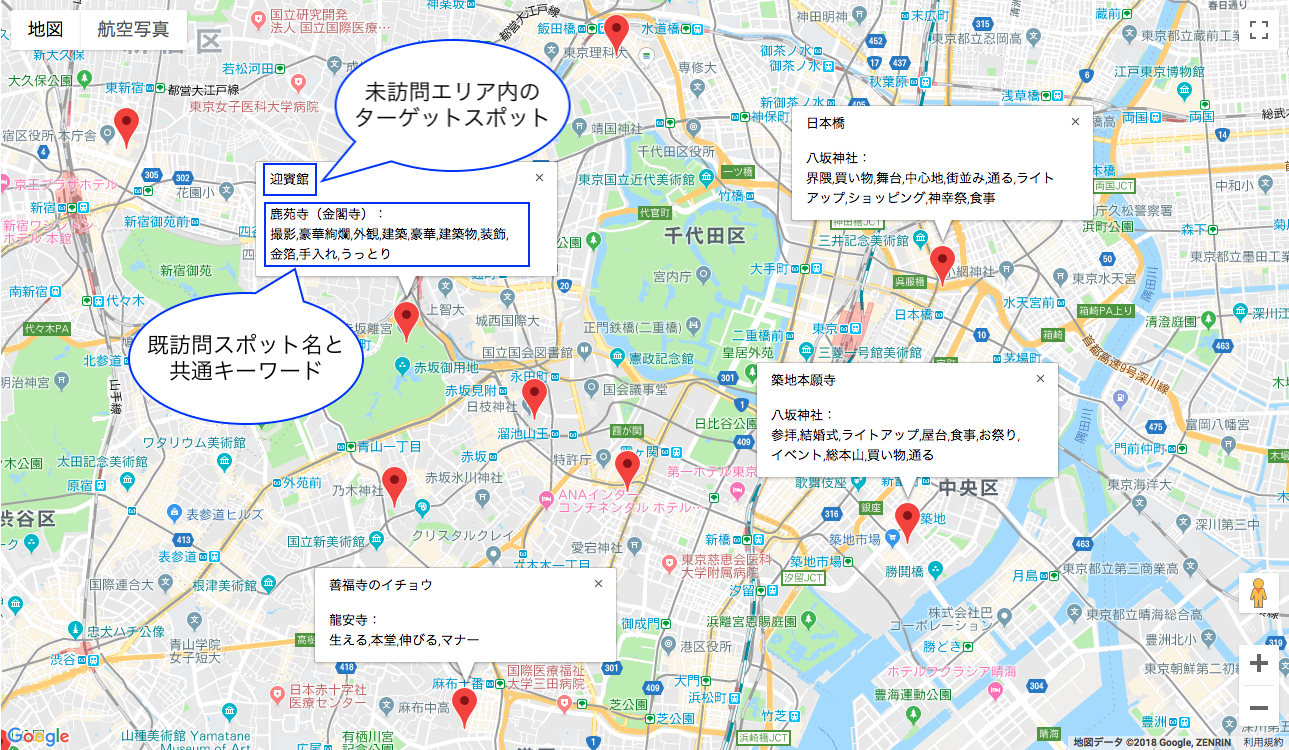
\includegraphics[width=0.9\textwidth]{./figure/map_jap.png}
    \caption{プロトタイプシステム}
    \label{fig:プロトタイプシステム}
   \end{center}
\end{figure}

%%%%%%%%%%%%%%%%%%%
\section{未訪問スポットと既訪問スポットの対応付け}
未訪問スポットを理解しやすくするために,最も位置付けの近いユーザの既訪問スポットを対応付ける手法を提案する.
まず,ユーザが既に訪問した複数個の観光スポットとこれから訪問したい観光スポットエリア情報を入力する.
本手法では,観光スポットのユーザレビューを用いて特徴ベクトルを生成する.
さらに,ユーザの観光地の位置付けを抽出するために,あるスポットに対し他の訪れたスポットと比較した相対的特徴ベクトルを算出する.
同様に,未訪問スポットもエリア内の各スポットの特徴ベクトルを求める.
また,未訪問エリアの各観光スポットの相対的特徴ベクトルを,そのエリアの他の観光スポットと比較して計算する.
次に,相対的特徴ベクトルの類似度によって既訪問スポットを未訪問スポットと対応付ける.
最後に,その関係性を説明するためのキーワードを抽出する.

%%%%%%%%%%%
\subsection{観光スポットのユーザレビューを用いた相対的特徴ベクトル生成}
2016年9月末までのじゃらんから得られたレビューデータを使用して,分散表現\cite{Le}を用いて観光スポットの特徴ベクトルを作成する.
このとき,観光スポット毎のレビューをまとめて1つの文書として扱う.
本研究では,分散表現を計算するためにPythonのライブラリであるgensim\footnote{https://radimrehurek.com/gensim/models/doc2vec.html}を利用する.
学習方法として,Distributed Bag-of-Wordsを利用して,各スポットの全レビューを使って300次元で作成したベクトルを使う.
既訪問スポットや未訪問スポットのレビューベクトルは,形態素解析器であるMeCab\cite{Kudo}に辞書「mecab-ipadic-NEologd」\footnote{https://github.com/neologd/mecab-ipadic-neologd/}用いて,分かち書きし原形にしたレビューを利用して作成する.

相対的特徴ベクトル$r_{state,i}$を,式\ref{math:Vector difference}として定義する.
\begin{equation}
  r_{state,i}=s_i-average(\{	s|s \in S_{state},s \neq s_i \})
  \label{math:Vector difference}
\end{equation}
相対的特徴ベクトルは,そのスポット自体の特徴ベクトルから他のスポットの特徴ベクトルの平均を引いた値によって得られる.
$S_{state} =\{s_1,s_2,\dots,s_n\}$は,既訪問スポットもしくは未訪問スポットのベクトル集合である.
$state$が$f$であれば,既訪問スポット集合を意味し,$state$が$u$であれば,未訪問スポット集合を意味する.
$s_i$は集合$S_{state}$内の観光スポット$i$の特徴ベクトルを示している.

%%%%%%%%%%%
\subsection{対応する観光スポットの決定と特徴語抽出}
未訪問エリア内のスポットを既訪問スポットと対応付ける.
具体的には,ある未訪問スポットの相対的特徴ベクトルに最も類似度が高い既訪問スポットを対応付ける.
類似度計算には,コサイン尺度を用いる.
ただし,類似度が閾値(本研究では0.125)以下である場合は対応付けを行わない.

スポットの対応関係を示すだけでは,どのような点で対応するのかを理解するのは難しい.
そこで,未訪問スポットと既訪問スポットの関係性を表すキーワードをユーザに提示する.
しかし,分散表現である相対的特徴ベクトルから単語の特徴を得ることはできないため,他の方法を用いて単語を抽出する.

すべてのレビューを\ref{subsec:スポットのレビューから相対的特徴ベクトル生成}節と同様に形態素解析器MeCabによって単語に分割する.
ただし,助詞,助動詞,連体詞,記号,ストップワードを削除している.

キーワード抽出手順について説明する.
まず,TFIDF法を使って対象となる既訪問スポットと未訪問スポットの特徴語とTFIDF値を求める.
IDF値を算出する集合は$S_{state}$を用いる.

2つのスポットに共通する特徴語のTFIDF値の調和平均を用いて,対応付けしたスポットの説明可能なキーワードとして抽出する.
各単語のスコアを式\ref{math:Harmonic Mean}によって定義する.
\begin{eqnarray}
  score(t,s_f,s_u) = \frac{2 \times tfidf(t,s_f) \times tfidf(t,s_u)}{tfidf(t,s_f) + tfidf(t,s_u)}
  \label{math:Harmonic Mean}
\end{eqnarray}
$tfidf(t,s_f)$と$tfidf(t,s_u)$は同じ単語に関する既訪問スポット$s_f$におけるTFIDF値と未訪問スポット$s_u$におけるTFIDF値を示している.
単語スコアの上位$N$個の単語を説明情報としてユーザに提示する.

%%%%%%%%%%%
\subsection{実行例}
\begin{table}[t]
  \caption{既訪問スポット集合と未訪問スポット集合}
  \label{table:既訪問スポット集合と未訪問スポット集合}
  \centering
  \begin{tabular}{l|l}
  \hline  \hline
  \multicolumn{1}{c|}{既訪問スポット名} & \multicolumn{1}{c}{未訪問スポット名} \\ \hline
  浅草寺                           & 東京ディズニーランド(R)                \\
  小田原城址公園                       & 新宿御苑                         \\
  伏見稲荷大社                        & 東京スカイツリー                     \\
  奈良公園                          & 東京タワー大展望台                    \\
  三島スカイウォーク                     & 明治神宮                         \\ \hline
  \end{tabular}
\end{table}

\begin{table*}[t]
    \caption{対応付け結果の例}
    \label{table:対応付け結果の例}
    \centering
    \begin{tabular}{l|l|l}
    \hline
    \multicolumn{1}{c|}{未訪問スポット} & \multicolumn{1}{c|}{既訪問スポット} & \multicolumn{1}{c}{特徴語}                                                                \\ \hline
    新宿御苑                         & 小田原城址公園                      & \begin{tabular}[c]{@{}l@{}}お花見,咲き誇る,園内,桜の時,のんびり,\\ 手入れ,自然,遊具,ツツジ\end{tabular}          \\ \hline
    東京スカイツリー                     & 三島スカイウォーク                    & \begin{tabular}[c]{@{}l@{}}富士山,揺れ,高所恐怖症,揺れる,天井,絶景,\\ エレベーター,パノラマ,展望デッキ,昇る\end{tabular} \\ \hline
    \end{tabular}
\end{table*}

表\ref{table:既訪問スポット集合と未訪問スポット集合}に示す,既訪問スポット集合と未訪問スポット集合を用いて対応付けを行った結果を説明する.
未訪問スポットは首都圏内を想定し5つのスポットを選んだ.
表\ref{table:対応付け結果の例}は,\ref{sec:未訪問スポットと既訪問スポットの対応付け}節で述べた提案手法を用いて抽出した対応付いたスポットの特徴語を示している.

未訪問スポット「新宿御苑」に対し,既訪問スポット「小田原城址公園」が対応付いた.
他に候補として「奈良公園」が考えられるが,「小田原城址公園」には花や遊具に対する記述が多く,「奈良公園」には鹿や草に対する記述が多い.
「新宿御苑」には花や遊具に対する記述が多いため,「小田原城址公園」と適切に対応付けたと考える.

未訪問スポット「東京スカイツリー」に対し「三島スカイウォーク」が対応づけられた.
どちらも眺めや高さに特徴があり関連付けられたと考えられる.
また,特徴語を見ると「富士山」が抽出されており,見える景色を想起させるような対応付けを行っていると考える.

%%%%%%%%%%%%%%%%%%%
\section{対応関係を表す特徴語抽出評価}

%%%%%%%%%%%
\subsection{実験内容}
提案手法のうちの特徴語抽出部分について評価を行うため,他のキーワード抽出手法と比較して評価を行う.
以下の3つの方法を比較する.
\begin{itemize}
  \item 算術平均法
  \item 乗算法
  \item 提案手法(調和平均)
\end{itemize}

\begin{table}[t]
  \caption{対応関係を表す特徴語の実験結果}
  \label{table:対応関係を表す特徴語の実験結果}
  \centering
  \begin{tabular}{c|r|r|r}
  \hline \hline
  選択肢 & \multicolumn{1}{c|}{算術平均} & \multicolumn{1}{c|}{乗算} & \multicolumn{1}{c}{提案手法} \\ \hline
  1  & 28.28\%                  & 31.31\%                  & 29.29\%                 \\
  2  & 35.35\%                  & 31.31\%                  & 35.35\%                 \\
  3  & 10.10\%                   & 14.14\%                  & 12.12\%                 \\
  4  & 26.26\%                  & 23.23\%                  & 23.23\%                 \\ \hline
  \end{tabular}
\end{table}

キーワードを抽出するとき,算術平均法では,2つのスポットに共通する特徴語のスコアとして算術平均を計算する.
抽出した単語のスコアを式\ref{math:Mean}によって定義する.
\begin{eqnarray}
  score(t,s_f,s_u) = \frac{tfidf(t,s_f) + tfidf(t,s_u)}{2}
  \label{math:Mean}
\end{eqnarray}

乗算法では,2つのスポットに共通する特徴語のスコアとして乗算を計算する.
抽出した単語のスコアを式\ref{math:Multi}によって定義する.
\begin{eqnarray}
  score(t,s_f,s_u) = tfidf(t,s_f) \times tfidf(t,s_u)
  \label{math:Multi}
\end{eqnarray}

%%%%%%%%%%%
\subsection{実験手順}
\label{subsec:実験手順}
クラウドソーシングのサービスである,CrowdWorks\footnote{https://crowdworks.jp/}を利用して23人の被験者を集めた.
まず,被験者は4から10個の自分が既に訪れたことのある観光スポットを入力した.
次に,被験者は旅行などで行ったことがなく,これから訪れたい都道府県やエリアを入力した.

本実験では,それぞれの手法において,対応付けられた既訪問スポットと未訪問スポット,およびスポット同士の関係を説明する特徴語を最大で5つまで提示した.
結果を評価するために,被験者は以下の4つの選択肢から1つを選んだ.
\begin{enumerate}
  \item 2つのスポットには関係性があり,キーワード\footnote{関係を説明する特徴語のことであるが,被験者には単にキーワードと示した.}によって関係が明確になった.
  \item 2つのスポットの関係性があり,キーワードによって初めて気がついた.
  \item 2つのスポットには関係性があるが,キーワードは関係を表していない.
  \item 2つのスポットには関係性がない.
\end{enumerate}

%%%%%%%%%%%
\subsection{実験結果と考察}
表\ref{table:対応関係を表す特徴語の実験結果}は,それぞれの手法における選択肢1から4それぞれの選択割合を示している.
乗算法では,多くの被験者が選択肢1を選択している.
このことから,乗算法は明らかな関係を表現する特徴語抽出ができることがわかった.
算術平均法と提案手法では,選択肢1の割合が減少し,選択肢2の割合が増加している.
このことから,算術平均法と提案手法は隠れた関係を表現する特徴語を見つけて被験者に提示することができると考えた.
しかし,算術平均法では,選択肢4の割合が増加しているため,提案手法より無関係な特徴語を抽出しやすくなったといえる.
また,選択肢1と2を合計すると,提案手法が最も高くなった.
このことから,スポットの関連を説明する特徴語抽出手法としては提案手法が妥当といえる.

%%%%%%%%%%%%%%%%%%%
\section{観光スポットの対応付けに関する評価}

%%%%%%%%%%%
\subsection{実験内容}
特徴語抽出については\ref{subsec:対応するスポットの決定と特徴語の抽出}節の手法を用いる.
提案手法のうちの対応付け部分について,以下の3つの手法を比較して評価を行う.
\begin{itemize}
  \item メタデータ法
  \item 分散表現法
  \item 提案手法
\end{itemize}

メタデータ法は,観光スポット検索サイトでスポットを検索するためのメタデータであるカテゴリ,滞在時間,訪問時期の一致を用いる.
まず,未訪問スポットに対し,すべてが一致する既訪問スポットを抽出する.
抽出できない場合は,季節,滞在時間,カテゴリの順に条件を緩和する.
既訪問スポットが複数ある場合は,レビュー数が最も多いスポットを選択する.
メタデータの例を以下に示す.
\begin{itemize}
 \item カテゴリ:神社・神宮・寺院,観光施設・名所巡り等
 \item 滞在時間:1時間未満,1--2時間等
 \item 訪問時期:1--12月,春,夏,秋,冬
\end{itemize}

分散表現法では,各スポットの特徴として\ref{subsec:スポットのレビューから相対的特徴ベクトル生成}節で作成した特徴ベクトルを使用する.
すなわち,式\ref{math:Vector difference}を用いずに,レビューから得た分散表現をそのまま用いる.

クラウドソーシングのサービスである,CrowdWorksを利用して24人の被験者を集めた.
実験手順は\ref{subsec:実験手順}節で説明した手順と同様である.

%%%%%%%%%%%
\subsection{実験結果と考察}
\begin{table}[t]
  \caption{対応付けに関する実験結果}
  \label{table:対応付けに関する実験結果}
  \centering
  \begin{tabular}{c|r|r|r}
  \hline \hline
  選択肢 & \multicolumn{1}{c|}{メタデータ} & \multicolumn{1}{c|}{分散表現} & \multicolumn{1}{c}{提案手法} \\ \hline
  1  & 41.30\%                    & 33.85\%                    & 29.36\% \\
  2  & 43.48\%                    & 47.69\%                    & 48.62\% \\
  3  & 2.17\%                     & 2.31\%                     & 2.75\% \\
  4  & 13.04\%                    & 16.15\%                    & 19.27\% \\
  \hline
  対応付け数  & 46                    & 130                    & 109 \\
   \hline
  \end{tabular}
\end{table}

対応付けしたスポットの合計数は285である.
表\ref{table:対応付けに関する実験結果}は,それぞれの方法における選択肢1から5それぞれの選択割合を示している.
メタデータ法について,多くの被験者が選択肢2を選択している.
このことから,メタデータ法は明らかな関係にあるスポット同士を関連付けることができることがわかった.
他の方法と比較して,提案手法では,選択肢1の割合が減少し,選択肢2の割合が増加している.
このことから,提案手法は隠れた関係を見つけて被験者に提示することができると考えた.
しかし,選択肢4の割合も増加しているため,無関係なスポットを抽出しやすくなったといえる.

選択肢1と2を合計すると,メタデータ法が最も高くなる.
このことから,説明するためのスポットの対応付けの精度が最も高いといえる.
しかし,メタデータ法は対応付けすることができるスポットの数が他の手法に比べ半分以下であり,未訪問スポットの多くに説明を付与することができない.

分散表現法と提案手法を詳細に考察するために,既訪問スポットの入力別に分析した.
入力した既訪問スポットの半数以上が同一カテゴリのスポットであった被験者(表中の「同じ場合」)とそうではない被験者(表中の「異なる場合」)に分けて集計した.
表\ref{table:既訪問スポットのカテゴリの同異による評価割合}は選択肢1と選択肢2の評価の割合である.
提案手法を使用すると,カテゴリが異なる場合において,分散表現法よりも選択肢1および選択肢2の割合を増加させることができる.
相対的特徴ベクトルを用いることによって,カテゴリをこえて各スポットの特徴を求めることができるといえる.
カテゴリが同じ場合の選択肢1は提案手法では,少なくなっている.
これは,相対的特徴ベクトルとしては,カテゴリの特徴が打ち消されたベクトルが生成されるため,明らかな関係となる対応付けが減ったと考えられる.
しかし,選択肢2が増えずに選択肢4が増え,無関係に見える対応付けを増やす結果となった.
そのため,入力スポットの種類によって対応付け手法を切り変えることが有効と考えられる.

\begin{table}[t]
  \caption{既訪問スポットのカテゴリの同異による評価割合}
  \label{table:既訪問スポットのカテゴリの同異による評価割合}
  \centering
  \begin{tabular}{c|c|r|r}
  \hline  \hline
  & 選択肢 & \multicolumn{1}{c|}{分散表現} & \multicolumn{1}{c}{提案手法} \\ \hline
  異なる場合                 & 1   & 19.23\%                  & 21.10\%                 \\ \cline{2-4}
  & 2   & 24.62\%                  & 25.69\%                 \\ \hline
  同じ場合                  & 1   & 14.62\%                  & 8.26\%                  \\ \cline{2-4}
  \multicolumn{1}{l|}{} & 2   & 23.08\%                  & 22.94\%                 \\ \hline
  \end{tabular}
\end{table}


%%%%%%%%%%%%%%%%%%%
\section{未訪問スポット説明の有効性評価}
%%%%%%%%%%%
\subsection{実験内容}
提案手法の有効性を評価するために以下の2つのシステムを使って比較する.
\begin{description}
  \item a.未訪問スポット名のみを表示
  \item b.未訪問スポット名,対応する入力スポット,対応を説明する特徴語を表示(提案手法)
\end{description}

被験者の入力は,これまでの実験と同様に,4個から10個の自分が既に訪れたことのある観光スポットと訪問したいエリアである.
ただし,エリアは2つ入力し,それぞれ別々にシステムa,システムbの入力として用いた.
なお,システムaとシステムbはランダムな順番で実行される.
システムを評価するために,被験者は以下の2つの設問について回答した.
また,それらの選択理由について自由記述で答えた.
\begin{description}
  \item Q1. 表示されたスポットの詳細情報はどちらの方が分かりやすいかを選択してください.
  \item Q2. 旅行の計画を立てる際にどちらの方が使いたいかを選択してください.
\end{description}

被験者はクラウドソーシングのサービスである,CrowdWorksを利用して集めた50人を用いた.

%%%%%%%%%%%
\subsection{実験結果と考察}
Q1に対する回答について,システムaとシステムbの結果はそれぞれ12件と38件となった.
被験者の回答理由の例を表\ref{table:システムaの方が良いと回答した被験者の自由記述}(システムa)および,表\ref{table:システムbの方が良いと回答した被験者の自由記述}(システムb)に示す.
また,
旅行の計画を立てる際にどちらの方が使いたいかに対する回答について,システムaとシステムbの結果はそれぞれ10件と40件となった.
被験者の回答より,得られた2つのシステムの特徴をまとめる.

システムbでは,キーワードや関連している情報が表示されており分かりやすいという特徴がある.
これに対し,システムaでは,スポット名のみが表示されているためシンプルで分かりやすいという特徴があるが,なぜそのスポットが検索されたのか分からないなどの否定的な回答も多数あった.
システムの表示情報が「シンプルな方が良い」と「詳細な情報が良い」の2つに大きく分けられているが,Q2の回答より80\%の被験者はシステムbの方が使いたいと回答しており,提案手法の方が評価が高いといえる.
また,システムbに関してスポットの写真を載せるとより分かりやすいなどの意見があり,画像による関連性の説明という拡張が考えられる.

\begin{table}[t]
  \caption{システムaの方が良いと回答した被験者の自由記述}
  \label{table:システムaの方が良いと回答した被験者の自由記述}
  \centering
  \begin{tabular}{l}
  \hline  \hline
  \begin{tabular}[c]{@{}l@{}}スポット名だけ書いてあるのでごちゃごちゃにならず、一目でどこに\\ 何があるか分かるからです.\end{tabular} \\ \hline
  スポットだけ表示されるところがシンプルで分かりやすかったから.                                                         \\ \hline
  シンプルにそのエリアの観光スポットを知ることが出来る.                                                             \\ \hline
  \end{tabular}
\end{table}

\begin{table}[t]
  \caption{システムbの方が良いと回答した被験者の自由記述}
  \label{table:システムbの方が良いと回答した被験者の自由記述}
  \centering
  \begin{tabular}{l}
  \hline  \hline
  自分が訪れた事のあるスポットと関連性があり連想しやすいから.                                                 \\ \hline
  \begin{tabular}[c]{@{}l@{}}どのような場所か想像しやすいので、計画を立てるのにも使いたい\\ と思ったから.\end{tabular} \\ \hline
  何と関連して表示された等詳細の情報が表示されわかりやすかった.                                                  \\ \hline
  \end{tabular}
\end{table}

%%%%%%%%%%%%%%%%%%%%%%%%%%%%%%%%%%%%%%%%%%
\chapter{地図上における未訪問スポットの説明性向上のための観光スポットの対応関係可視化手法}
%%%%%%%%%%%%%%%%%%%%%%%%%%%%%%%%%%%%%%%%%%
本章では,観光スポット間の対応関係を地図上に可視化する手法を提案する.
また,プロトタイプシステムを構築し,既訪問スポットと未訪問スポットの説明性向上のための観光スポットの対応関係を地図上に可視化した効果を評価する実験を行う.

%%%%%%%%%%%%%%%%%%%
\section{概要}
近年,ユーザはWeb上の観光情報を活用して旅行計画を立てることが多くなっている.
しかし,旅行は一般的に訪れたことがないスポットに行くことが多いため,観光情報を適切に理解することは困難である.
そこで,訪問したことがある観光スポットの特徴を用いて,未訪問エリアの観光スポットを対応付けして,ユーザの未知なスポットに対する理解を支援することを考える.
観光スポット間の対応関係を地図上に可視化する手法を提案する.
本手法では,まず,スポットの特徴ベクトル間の類似度に基づいて既訪問スポットと未訪問スポットを対応付けし,その対応関係を説明するための特徴語を抽出する.
次に,地図上で表示するための意味的な位置関係を決定する.
具体的には,未訪問スポットからの距離と類似度によって存在確率を決定して,意味的な位置関係に基づいて観光スポットの対応関係をわかりやすくするための既訪問スポットの座標を算出する.
また,プロトタイプシステムを構築し,既訪問スポットと未訪問スポットの説明性向上のための観光スポットの対応関係を地図上に可視化した効果を評価する実験を行う.

%%%%%%%%%%%%%%%%%%%
\section{観光スポット間の対応関係を用いた可視化}
未訪問スポットを理解しやすくするために,もっとも位置付けの近いユーザの既訪問スポットを対応付ける手法を提案した\cite{潘}.
この手法では,ユーザが既に訪問した複数個の観光スポットとこれから訪問したい観光エリアを入力とする.
ユーザが入力した観光スポット集合のユーザレビューを用いてそれぞれのスポットの特徴ベクトルを生成する.
同様に,未訪問スポットもエリア内の各スポットの特徴ベクトルを求める.
次に,特徴ベクトルのコサイン類似度によって既訪問スポットを未訪問スポットと対応付ける.
最後に,その関係性を説明するためのキーワードをTF-IDF特徴量と調和平均で抽出する.

ある未訪問スポットに対して,入力した既訪問スポットがどのような関係にあるのか地図上で,一目で把握できることが望ましい.
ユーザは地図上で未訪問スポットを検索しているものとし,まず,地図上の実際にスポットが存在する座標に未訪問スポットを配置する.
次に,既訪問スポットの位置を決定する.
これは未訪問スポットとの対応関係によって変化し,未訪問スポットとの類似度が高いと近く,類似度が低いと遠くなるように配置することで,意味的な位置関係を表現する.
既訪問スポットの座標は,式\ref{math:score}によって求める.
\begin{eqnarray}
Score(s_f,T) = \sum_{s_u \in S_u}^{} w(s_u,s_f) \times P_{s_u,s_f}(d(s_u,T))
    \label{math:score}
\end{eqnarray}
$S_u$を未訪問エリア内のスポット集合とする.
$w(s_u,s_f)$は,ある既訪問スポット$s_f$と未訪問スポット$s_u$の類似度が正であれば$1.0$,負であれば$-0.5$を返す関数である.
$T$は,候補の座標である.
$d(s_u,T)$は,ある座標$T$から未訪問スポット$s_u$のユークリッド距離である.
また,$P_{s_u,s_f}$は,平均$\mu$が$0$,標準偏差$\sigma$が$(1-|cos(vec(s_u),vec(s_f))|) \times \alpha$である正規分布を表す.
$\alpha$は$1$である.
$vec$は未訪問スポットや既訪問スポットの特徴ベクトルを返す関数である.
$Score(s_f,T)$がもっとも大きな座標$T$を既訪問スポットの座標とする.
図\ref{fig:image}は既訪問スポットの経度座標計算の例である.
縦軸はスコアの値であり,横軸は経度である.
4つの未訪問スポットを用いて,$Score(s_f,T)$(合計スコア)を計算している.
その結果,$135.06$の座標がもっとも高くなる.
緯度についても同様に行う.
本稿では,近似として対象エリア内でランダムに200個の$T$を作り,それを用いた.

\begin{figure}[t]
  \begin{center}
    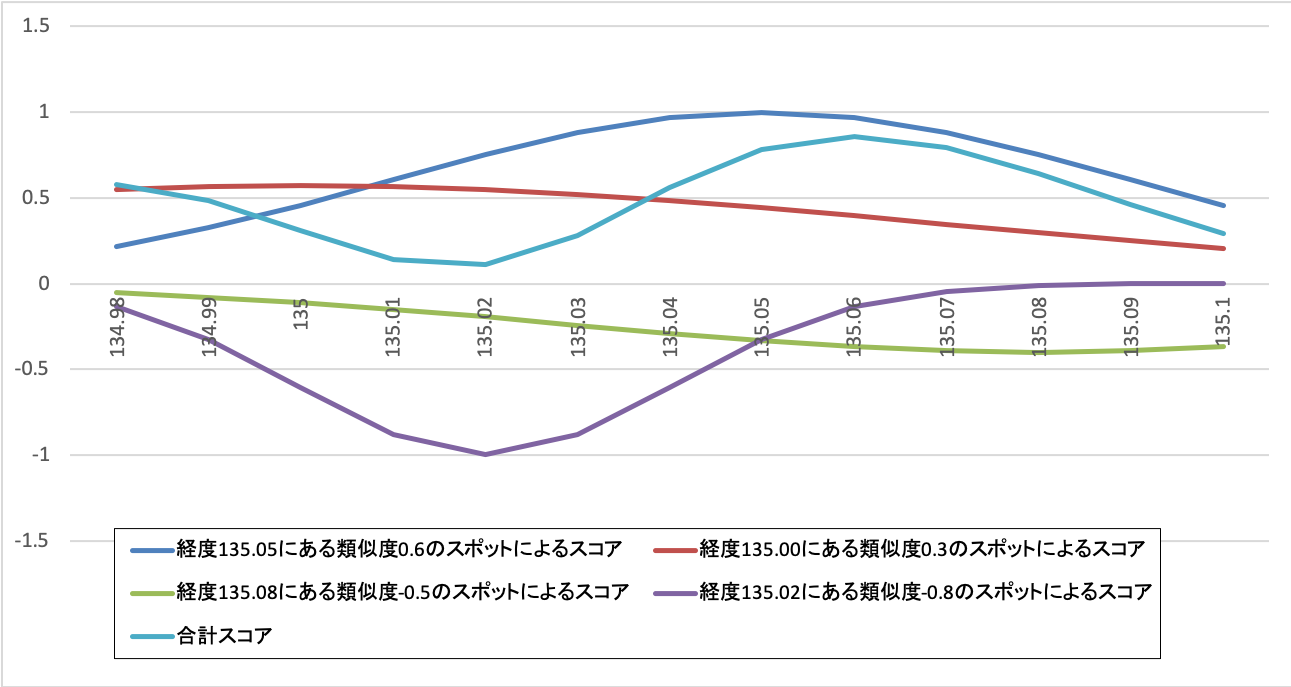
\includegraphics[width=0.9\textwidth]{./figure/score_image.png}
    \caption{既訪問スポットの経度座標計算の例}
    \label{fig:image}
   \end{center}
\end{figure}

%%%%%%%%%%%%%%%%%%%
\section{対応関係の可視化評価}

%%%%%%%%%%%
\subsection{実験内容}
未訪問スポットの説明性向上のための観光スポットの対応関係可視化手法の評価を行うため,以下の3つの提示手法を使って比較する.
図\ref{fig:P},図\ref{fig:L},図\ref{fig:T}は3つの提示手法それぞれのプロトタイプシステムとなっている.
黒いピンは入力した既訪問スポット,赤いピンは未訪問エリア内のスポットを意味している.
表示が重なることもあるため,黒いピンをクリックすると既訪問スポット名を吹き出しでも表示する.
また,3つの提示手法において,類似度が「0.0」以下であれば,関係を表現するキーワードが「なし」と表示する.
これは負の関係を表すキーワードは一般的に理解しにくいためである.
\begin{figure*}[t]
	\centering
	\begin{minipage}{.35\textwidth}
		\centering
		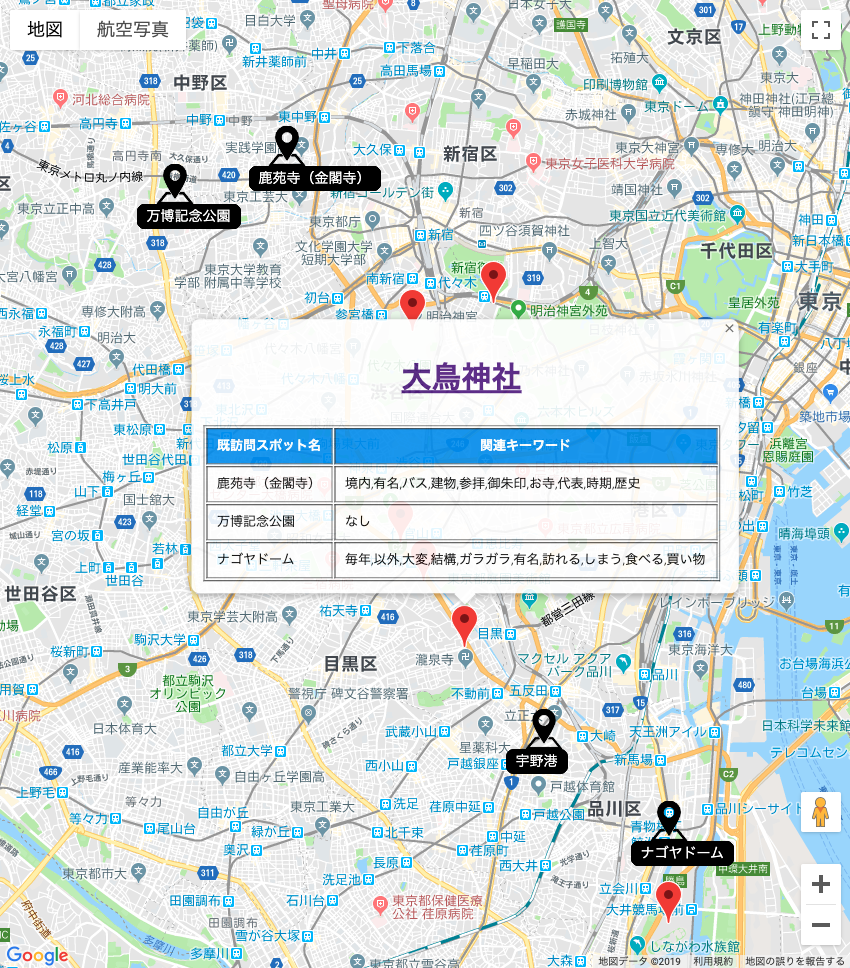
\includegraphics[clip, width=5cm]{./figure/position_map.png}
		\caption{位置関係($Position\_Map$)}
		\label{fig:P}
	\end{minipage}
	%
	\hfil
	%
	\begin{minipage}{.35\textwidth}
		\centering
		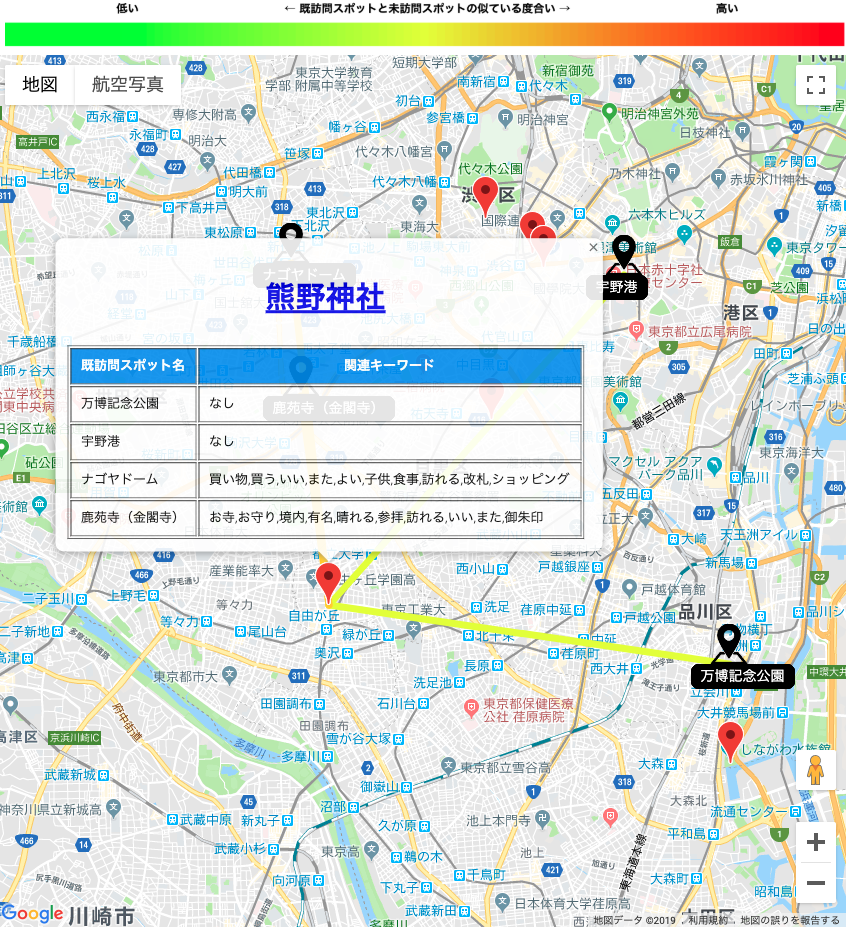
\includegraphics[clip, width=5cm]{./figure/line_map.png}
		\caption{位置関係+線($Line\_Map$)}
		\label{fig:L}
	\end{minipage}
	\hfil
	%
	\begin{minipage}{.35\textwidth}
		\centering
		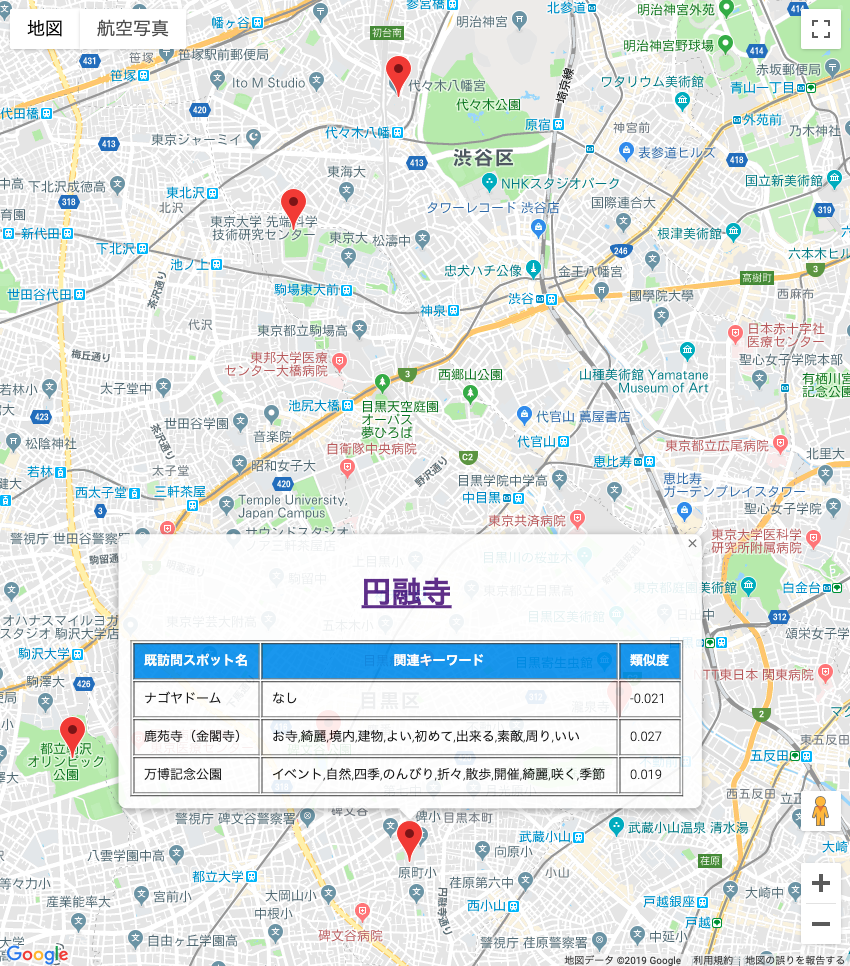
\includegraphics[clip, width=5cm]{./figure/table_map.png}
		\caption{表形式($Table\_Map$)}
		\label{fig:T}
	\end{minipage}
\end{figure*}


$Position\_Map$(図\ref{fig:P})では,検索対象のスポットと既訪問スポットの関連度を全体的な位置関係で表現している.
既訪問スポットは実際の座標ではなく,提案手法で決定した座標で表示される.
赤いピンをクリックすると詳細情報が表示される.
詳細情報は,未訪問スポット名,対応する既訪問スポット名,未訪問スポットと既訪問スポットの関係を表現するキーワードである.

$Line\_Map$(図\ref{fig:L})では,位置関係による提示に加えて線の色を使って表現している.
線の色は赤いピンと黒いピンの類似度を示している.
線は緑色に近いと類似度が低く,赤色に近いと類似度が高いことを意味している.
赤いピンをクリックすると詳細情報が表示される.
詳細情報は,$Position\_Map$と同じく,未訪問スポット名,対応する既訪問スポット名,未訪問スポットと既訪問スポットの関係を表現するキーワードである.

$Table\_Map$(図\ref{fig:T})では,位置関係や線は用いずに,$Line\_Map$で表現していたすべての情報を表形式でまとめて表現している.
詳細情報は,現在選択している未訪問スポット名と,対応する既訪問スポット名,未訪問スポットと既訪問スポットの関係を表現するキーワード,類似度である.
類似度の値は「-1.0から1.0」の間になる.
「-1.0」はもっとも類似せず,「1.0」はもっとも類似することを意味している.

%%%%%%%%%%%
\subsection{実験手順}
クラウドソーシングのサービスである,CrowdWorksを利用して75人合計120件のデータを集めた.
まず,被験者は3個から9個の自分が既に訪れたことのある,かつ気に入った観光スポットを入力した.
次に,被験者は旅行などで行ったことがなく,これから訪れたい都道府県やエリアを入力した.

本実験では,各提示手法において,検索スポットが重複しないように振り分け,3つの提示手法を連続して利用した.
それぞれの提示手法において,被験者は検索スポットから行き先を決定した.
このとき,表示順に影響をなくすために,6パターンの表示順を作成し,被験者はランダムに1つの表示順で実験を行う.
実験を行った後,以下の項目について評価する.
\begin{itemize}
  \item 各提示手法の行き先の決定しやすさ
  \item $Position\_Map$と$Line\_Map$どちらのほうが,訪問履歴との関係がわかりやすかったか
  \item $Line\_Map$と$Table\_Map$どちらのほうが,訪問履歴との関係がわかりやすかったか
  \item 各提示手法の訪問先決定までにかかった体感時間
  \item 各提示手法の訪問先決定までにかかった労力
\end{itemize}
また,それぞれの手法について,自由記述で意見を書いてもらった.

%%%%%%%%%%%
\subsection{実験結果と考察}
\begin{table}[t]
    \caption{行き先の決定しやすさの回答数割合}
    \label{table:行き先の決定しやすさ}
    \centering
    \begin{tabular}{l|rrrrr|l}
    \hline
    決定しやすさ   & \multicolumn{1}{l}{1} & \multicolumn{1}{l}{2} & \multicolumn{1}{l}{3} & \multicolumn{1}{l}{4} & \multicolumn{1}{l|}{5} & 平均    \\ \hline
    $Position\_Map$ & 5.0\%                & 15.8\%               & 15.0\%               & 51.7\%               & 12.5\%                & 3.51 \\
    $Line\_Map$     & 2.5\%                & 12.5\%               & 19.2\%               & 50.0\%               & 15.8\%                & 3.64 \\
    $Table\_Map$    & 3.3\%                & 5.8\%                & 35.0\%               & 46.7\%               & 9.2\%                 & 3.53 \\ \hline
    \end{tabular}
\end{table}
表\ref{table:行き先の決定しやすさ}は3つの提示手法それぞれの行き先の決定しやすさを5段階評価した回答数である.
5はとても決定しやすい,1はとても決定しづらいを意味している.
表\ref{table:行き先の決定しやすさ}の平均値から$Line\_Map$がもっとも決定しやすいことがわかった.
$Line\_Map$は$Position\_Map$より決定しやすい理由として,$Line\_Map$は位置情報提示に加えて,線を描くことによって,より既訪問スポットと未訪問スポットの対応関係を表現することができたためと考えられる.
ただし,3つの提示手法について$t$検定を行った結果,それぞれ有意差があるとはいえなかった.

\begin{table}[t]
    \caption{$Position\_Map$と$Line\_Map$の訪問履歴との関係の回答数割合}
    \label{table:PLの訪問履歴との関係}
    \centering
    \begin{tabular}{l|r}
    \hline
    回答    & 回答数の割合 \\
    \hline
    $Position\_Map$がわかりやすかった   & 15.8\% \\
    $Position\_Map$がややわかりやすかった & 28.3\% \\
    どちらでもない                  & 20.0\% \\
    $Line\_Map$がややわかりやすかった     & 24.2\% \\
    $Line\_Map$がわかりやすかった       & 11.7\% \\ \hline
    \end{tabular}
\end{table}
\begin{table}[t]
    \caption{$Line\_Map$と$Table\_Map$の訪問履歴との関係の回答数割合}
    \label{table:LTの訪問履歴との関係}
    \centering
    \begin{tabular}{l|r}
    \hline
    回答    & 回答数の割合 \\
    \hline
    $Line\_Map$がわかりやすかった    & 12.5\% \\
    $Line\_Map$がややわかりやすかった  & 28.3\% \\
    どちらでもない               & 27.5\% \\
    $Table\_Map$がややわかりやすかった & 24.2\% \\
    $Table\_Map$がわかりやすかった   & 7.5\%  \\ \hline
    \end{tabular}
\end{table}
表\ref{table:PLの訪問履歴との関係}は$Position\_Map$と$Table\_Map$どちらのほうが,訪問履歴との関係がわかりやすかったかの回答数の割合となっている.
表\ref{table:PLの訪問履歴との関係}から$Position\_Map$がわかりやすいの割合が$44.2\%$に対して,$Line\_Map$が$35.8\%$のため,$Position\_Map$のほうがわかりやすいといえる.
一方,表\ref{table:行き先の決定しやすさ}では,$Position\_Map$がもっとも決定しづらいといえる.
理由として,$Position\_Map$は他の2つの提示手法と比べると,決定しづらい回答数が多くなっている.
また,「黒いピンと赤いピンの類似距離という関係性があまりよくわかりません」といった意見の被験者が多数おり,強く好まない被験者が一定数が存在するため,このような結果となったと考える.
位置関係を表現する際に,仮想的な地物の類似性を視覚的に表していることが明確にわかるインタフェースにする必要がある.
また,表\ref{table:LTの訪問履歴との関係}は$Line\_Map$と$Table\_Map$の訪問履歴との関係のわかりやすさの回答数の割合となっている.
表\ref{table:LTの訪問履歴との関係}から$Line\_Map$がわかりやすいの割合が$40.4\%$に対して,$Table\_Map$が$31.7\%$のため,$Line\_Map$のほうがわかりやすい.

\begin{table}[t]
    \caption{$Position\_Map$と$Line\_Map$の決定しやすさと関係わかりやすさについての回答数}
    \label{table:決定しやすさと関係わかりやすさについての回答数}
    \centering
    \begin{tabular}{l|l|r}
    \hline
    決定のしやすさ     & 関係のわかりやすさ      & \multicolumn{1}{l}{回答数} \\ \hline
    $P$は$L$よりしやすい & $P$が$L$よりわかりやすい & 18                       \\
    $L$は$P$よりしやすい & $P$が$L$よりわかりやすい & 3                        \\
    $P$は$L$よりしやすい & $L$が$P$よりわかりやすい & 1                        \\
    $L$は$P$よりしやすい & $L$が$P$よりわかりやすい & 23                       \\ \hline
    \end{tabular}
\end{table}
表\ref{table:決定しやすさと関係わかりやすさについての回答数}は同一の被験者の表\ref{table:行き先の決定しやすさ}と表\ref{table:PLの訪問履歴との関係}の結果を比較し,$Position\_Map$と$Line\_Map$の行き先の決定しやすさと訪問履歴との関係のわかりやすさについての回答数となっている.
表\ref{table:行き先の決定しやすさ}に関しては,どちらに大きな値をつけたかを集計している.
行き先決定のしやすさと訪問履歴の互いの影響に関して,決定しやすさと訪問履歴の評価が一致で回答した数はが異なると回答した数より多いため,互いに影響があることが考えられる.
% また,行き先決定のしやすさに関してて$Line\_Map$のほうが決定しやすいと回答する数が多い.
% 訪問履歴との関係に関して$Position\_Map$のほうが関係がわかりやいと回答する数が多い.

\begin{table}[t]
    \caption{訪問先決定までにかかった体感時間の回答数割合}
    \label{table:訪問先決定までにかかった体感時間}
    \centering
    \begin{tabular}{l|rrrrr|r}
    \hline
                  & \multicolumn{1}{l}{1} & \multicolumn{1}{l}{2} & \multicolumn{1}{l}{3} & \multicolumn{1}{l}{4} & \multicolumn{1}{l|}{5} & \multicolumn{1}{l}{平均} \\ \hline
    $Position\_Map$ & 10.0\%               & 40.8\%               & 30.0\%               & 15.8\%               & 3.3\%                & 2.62                   \\
    $Line\_Map$     & 13.3\%               & 35.8\%               & 30.0\%               & 15.8\%               & 5.0\%                & 2.63                   \\
    $Table\_Map$    & 9.2\%                & 33.3\%               & 35.8\%               & 18.3\%               & 3.3\%                & 2.73                   \\ \hline
    \end{tabular}
\end{table}

\begin{table}[t]
    \caption{訪問先決定までにかかった労力の回答数割合}
    \label{table:訪問先決定までにかかった労力}
    \centering
    \begin{tabular}{l|rrrrr|r}
    \hline
                  & \multicolumn{1}{l}{1} & \multicolumn{1}{l}{2} & \multicolumn{1}{l}{3} & \multicolumn{1}{l}{4} & \multicolumn{1}{l|}{5} & \multicolumn{1}{l}{平均} \\ \hline
    $Position\_Map$ & 14.2\%               & 35.8\%               & 27.5\%               & 16.7\%               & 5.8\%                 & 2.64                   \\
    $Line\_Map$     & 15.8\%               & 36.7\%               & 30.0\%               & 12.5\%               & 5.0\%                 & 2.54                   \\
    $Table\_Map$    & 11.7\%               & 33.3\%               & 34.2\%               & 15.8\%               & 5.0\%                 & 2.69                   \\ \hline
    \end{tabular}
\end{table}

表\ref{table:訪問先決定までにかかった体感時間}は3つ提示手法それぞれの訪問先を決定するまでにかかった体感時間を5段階評価した回答数である.
1は訪問先決定するまでに短い時間で,5は長い時間で決定していることを意味している.
表\ref{table:訪問先決定までにかかった労力}は3つ提示手法それぞれの訪問先決定するまでにかかった労力を5段階評価した回答数である.
1は訪問先決定するまで少ない労力で,5は多い労力で決定していることを意味している.
体感時間と労力の相関係数を計算すると$0.74$と強い正の相関があり,体感時間が短いと労力も少なく,体感時間が長いと労力も多くなる.
% 表\ref{table:訪問先決定までにかかった体感時間}と表\ref{table:訪問先決定までにかかった労力}から$Table\_Map$がもっとも被験者にとって手間がかかっていることがわかる.
訪問先決定までにかかった体感時間が短いと回答した数の割合は$Position\_Map$が$50.8\%$,$Line\_Map$が$49.2\%$,$Table\_Map$が$42.5\%$となっている.
よって,$Position\_Map$がかかった体感時間がもっとも短く,$Table\_Map$がもっとも長いことがわかった.
訪問先決定までにかかった労力が少ないと回答した数の割合は$Position\_Map$が$50.0\%$,$Line\_Map$が$52.5\%$,$Table\_Map$が$45.0\%$となっている.
よって,$Line\_Map$がかかった労力がもっとも少ない,$Table\_Map$がもっとも多いことがわかった.
以上から,$Line\_Map$は体感時間が短くかつ労力も少なく訪問先を決定することができ,$Table\_Map$はもっとも被験者にとって手間がかかっていることがわかった.
対応関係を位置情報で表すことによって,表形式の時間と労力の問題点について改善することができるといえる.
$Line\_Map$は被験者に提示する文字の情報を少なくして,線の色と位置関係を使って既訪問スポットと未訪問スポット対応関係を見せることによって,他の2つの提示手法と比べると理解容易化することができたと考えられる.


%%%%%%%%%%%%%%%%%%%%%%%%%%%%%%%%%%%%%%%%%%
\chapter{考察}
%%%%%%%%%%%%%%%%%%%%%%%%%%%%%%%%%%%%%%%%%%


%%%%%%%%%%%%%%%%%%%%%%%%%%%%%%%%%%%%%%%%%%
\chapter{結論}
%%%%%%%%%%%%%%%%%%%%%%%%%%%%%%%%%%%%%%%%%%



%%%%%%%%%%%%%%%%%%%%%%%%%%%%%%%%%%%%%%%%%%
% 謝辞
\acknowledge{謝辞}
%%%%%%%%%%%%%%%%%%%%%%%%%%%%%%%%%%%%%%%%%%
修士課程での研究全般に渡ってご指導賜りました北山大輔准教授に厚く御礼申し上げます.

お忙しい中貴重な時間を割いて副指導教員およぶ副査を引き受けてくださり,ご指導賜りました三木良雄教授に感謝致します.

同様に,お忙しい中貴重な時間を割いて副査を引き受けてくださり,ご指導賜りました〇〇教授に感謝致します.

% また,学士学位論文に関するご指導も含め,3年間に渡ってご指導賜りました北山大輔准教授に感謝致します.
研究室配属からの3年間に渡って,切磋琢磨し心の支えにもなってくれた歴代のインタラクティブメディア研究室メンバ全員に感謝致します.

最後に,名前を書き切ることはできませんが,両親をはじめ,私のこれまでの人生を支えてくださった全ての方に心から感謝いたします.
ありがとうございました.


%%%%%%%%%%%%%%%%%%%%%%%%%%%%%%%%%%%%%%%%%%
% 参考文献
\references{参考文献}%タイトル変更可能
%%%%%%%%%%%%%%%%%%%%%%%%%%%%%%%%%%%%%%%%%%
\bibliographystyle{junsrt}
\bibliography{man}
%bibtexを使う方は,以下をコメントアウトし,上記を有効にする。スタイルは適宜変更のこと。
% \begin{thebibliography}{99}
%     \bibitem{c1} (雑誌の場合;雑誌とは論文誌等のこと)著者名, ``標題, '' 雑誌名, 巻, 号, pp.A--B, Month, 年.
%     \bibitem{c2} (著書,編書の場合)著者名, 書名, 編者名, 発行所, 発行都市名, 発行年.
%     \bibitem{c3} (著書の一部を引用する場合)著者名, ``標題, '' 書名, 編者名, 章番号またはpp.A--B, 発行所, 発行都市名, 発行年.
%     \bibitem{c4} (国際学会論文集の場合)著者名, ``標題, '' 会議名, no.A, pp.B--C, 都市名, 国名, Month, 年.
%     \bibitem{c5} (国内学会,研究会論文集の場合)著者名, ``標題, '' 学会論文集名, vol.A, no.B, pp.C--D, 都市名, 国名, Month, 年.
%     \bibitem{Kurashima}
%         T. {Kurashima}, T. {Iwata}, G. {Irie} and K. {Fujimura},
%         ``Travel Route Recommendation Using Geotags in Photo Sharing Sites,"
%         In Proceedings of the 19th ACM International Conference on Information and Knowledge Management,
%         pp.579-588, 2010
%     \bibitem{Kurashima}
%         R. {Kitamura} and T. {Itoh},
%         ``Tourist Spot Recommendation Applying Generic Object Recognition with Travel Photos,"
%         In 2018 22nd International Conference Information Visualisation (IV),
%         pp.1-5, 2018
%     \bibitem{Cheng}
%         A.J. {Cheng}, Y.Y. {Chen}, Y.T. {Huang} and W.H. {Hsu},
%         ``Personalized travel recommendation by mining people attributes from community-contributed photos,"
%         In Proceedings of the 19th ACM international conference on Multimedia,
%         pp.83-92, 2011
%     \bibitem{松本}
%         松本 敦志, 杉本 徹,
%         ``クチコミから抽出した特徴語を利用する観光地検索支援,"
%         第75回全国大会講演論文集,
%         vol.2013, no.1, pp.307-308, 2013
% \end{thebibliography}



%%%%%%%%%%%%%%%%%%%%%%%%%%%%%%%%%%%%%%%%%%%%%%%%%%%%%%
% 発表実績
\publications{本研究に関する発表}
%%%%%%%%%%%%%%%%%%%%%%%%%%%%%%%%%%%%%%%%%%%%%%%%%%%%%%
\begin{thepublication}
%
\publicationtype{論文}
\item \underline{潘健太}, 北山大輔, ``説明性向上のためのユーザレビューを用いた観光スポットの対応付け手法," 情報処理学会論文誌データベース, 第84号, 2019.
%
\publicationtype{査読付き会議}
\item \underline{Kenta Han}, Daisuke Kitayama, ``An Explanation Method of Unfamiliar Tourist Spots based on Roles of User's Familiar Spots," Lecture Notes in Engineering and Computer Science: Proceedings of The International MultiConference of Engineers and Computer Scientists 2019, Hong Kong, pp358-362, 13-15 March, 2019.
%
\publicationtype{研究会}
\item \underline{潘健太}, 北山大輔, ``ユーザの既訪問スポットの位置付けに基づく未訪問スポットの説明手法," 第11回データ工学と情報マネジメントに関するフォーラム(DEIM Forum 2019), H7-2, 2019
\item \underline{潘健太}, 北山大輔, ``地図上における未訪問スポットの説明性向上のための観光スポットの対応関係可視化手法," 観光情報学会第20回研究発表会, 2019
%
% \publicationtype{全国大会}
% \item \underline{1st Author}, 2nd Author, 3rd Author, Last Author, ``Title,'' Conference, Year.
%
\end{thepublication}


%%%%%%%%%%%%%%%%%%%%%%%%%%%%%%%%%%%%%%%%%%%%%%%%%%%%%%
% その他の発表実績
\publications{その他の発表実績}
%%%%%%%%%%%%%%%%%%%%%%%%%%%%%%%%%%%%%%%%%%%%%%%%%%%%%%
\begin{thepublication}
\publicationtype{研究会}
\item \underline{潘健太}, 北山大輔, ``ユーザのレビュー選択に基づく観光スポット検索手法," 第10回データ工学と情報マネジメントに関するフォーラム(DEIM Forum 2018), H1-2, 2018
\item \underline{潘健太}, 北山大輔, ``観光スポット検索のためのユーザのレビュー選択と特徴抽出に関する考察," 電子情報通信学会技術研究報告, vol. 118, no. 107, DE2018-5, pp. 21-24, 2018
\end{thepublication}


%%%%%%%%%%%%%%%%%%%%%%%%%%%%%%%%%%%%%%%%%%%%%%%%%%%%%%
% 受賞
\publications{受賞}
%%%%%%%%%%%%%%%%%%%%%%%%%%%%%%%%%%%%%%%%%%%%%%%%%%%%%%
\begin{thepublication}
\publicationtype{査読付き会議}
\item \underline{Kenta Han}, Daisuke Kitayama, ``An Explanation Method of Unfamiliar Tourist Spots based on Roles of User's Familiar Spots," Lecture Notes in Engineering and Computer Science: Proceedings of The International MultiConference of Engineers and Computer Scientists 2019, Hong Kong, pp358-362, 13-15 March, 2019.
\end{thepublication}


%%%%%%%%%%%%%%%%%%%%%%%%%%%%%%%%%%%%%%%%%%%%%%%%%%%%%%
% 研究室内部用の資料
\begin{domestic}
%%%%%%%%%%%%%%%%%%%%%%%%%%%%%%%%%%%%%%%%%%%%%%%%%%%%%%
\chapter{ファイルの場所}
本論文のファイル一式は研究室共有の...に保存してあります。実験プロジェクト等は研究室共有の...に保存してあります。


\chapter{引き継ぎ資料}
実験プロジェクトの使用法や,その他端書きは研究室共有の...に保存してあります。



%%%%%%%%%%%%%%%%%%%%%%%%%%%%%%%%%%%%%%%%%%
% 文書の終わり
%%%%%%%%%%%%%%%%%%%%%%%%%%%%%%%%%%%%%%%%%%
\end{domestic}
\eof%End-Of-File
%%%\end{document}は不要です
